% Chapter 1

\chapter{Implementation} % Chapter title

\label{ch:theory} % For referencing the chapter elsewhere, use \autoref{ch:introduction} 

%----------------------------------------------------------------------------------------

As mentioned previously the work was divided into a series of phases. Before these commenced, we wanted to decide on which tools we were going to use for the application. 
We knew we wanted to make an online application that would enable a user to model the flooding of a provided area.  
To model the flood we decided on using GRASS at it is a powerful Open Source software, with a history being used in a variety of professional settings – such as the american army corps of engineers. Furthermore, the application allows easy access to it's core functions through a Python interface. 
GRASS is natively supported by the WPS called PyWPS. Therefore this seemed like a natural choice for our project. 
To gain the online application of the project, a web server would obviously be needed, and for this hosting of some sort, and we ended up using the Amazon Elastic Compute Cloud (or EC2) for this purpose.
The majority of the development was performed on machines running Ubuntu, so the syntax and explanations will therefore reflect this fact.
Now that we were set on the tools we were going to use, we were starting the actual implementation, we decided to sketch out how we expected the application would end up looking, and functioning.\\
\\

IMAGE OF THIS\\
\\

Now that we have a rough idea of how the project would be working, we could get started on implementing these ideas into an actual solution.

\section{Phase 1}
This phase involved setting up all the necessary preliminary settings, such as our local and server-side GRASS installations, the needed environment variables, and setting up a server. \\

\paragraph{Setting up a local scripting environment:} Instead of working directly on the server, and working with PyWPS we decided to create a local working environment using GRASS with Python, on our own machines. This was done to simplify the workflow and make sure that  we didn't have to update the server whenever changes were made to the code. \\
The syntax for running GRASS through Python and GRASS through the WPS differ, so it would have to be changed accordingly when porting it online, but this would allow us to get started immediately. \\
When working with GRASS, but not explicitly starting a GRASS session, a variety of environment variables have to be set. 

\begin{itemize}
\item \textsc{GISBASE}: This points to the top level directory of the GRASS installation
\item \textsc{GISDBASE}: GRASS' database location, usually initiated as grassdata.
\item \textsc{PATH}: The path location of GRASS, usually includes /script/ and /bin/.
\end{itemize} \\

These settings are set up in the header of the project, and for our set up look like this:

\begin{lstlisting}[language=Python]
gisbase = '/usr/lib/grass70'
os.environ['GISBASE'] = gisbase
os.environ['PATH'] += os.pathsep + os.path.join(gisbase, 'extrabin')
os.environ['GISDBASE'] = gisdb
\end{lstlisting}

When running the python script, it now initiates the GRASS environmental variables that are necessary for importing and using GRASS' functions.\\

\paragraph{Setting up the server:}Before being able to set up PyWPS, it is necessary to set up a server, capable of serving the processing service.  
As PyWPS was created with Linux in mind, and because the creators even specify that it works better on a Linux-based operating system, we wanted to make sure that the server was running this as well. Today there are a variety of different hosting services available, but for this project it was decided to use Amazon Web Services (AWS).\\

The main reason for running the server on this service is because several members of the group have had previous experience with launching minor applications on this platform, but also because it is possible to launch a so-called micro instance, which is free for the first year. The free-tier provides a very basic server, with little processing power and hard drive space – but for a proof-of-concept project such as this, it would suffice. \\
Initiating a server on Amazon's Elastic Compute Cloud (EC2) is easy, and only takes a couple of minutes. As several members of the group were already using the Linux-based operating system Ubuntu we decided to base the server this.\\
Connecting to your server is done using SSL, and when using Ubuntu, can be performed with the terminal. The only situation where this would not be so, is when having to upload specific files, for this a FTP client software is used.

\paragraph{Setting up Apache:}Every instance set up with Amazon, is provided with an IP address which can be used to visit the server using a browser. The Ubuntu image installed on the server did not contain a pre-installed web server, so it was necessary to install and configure this first.
Installing software on a machine running Linux is, and Ubuntu uses the package manager aptitude. Using the following terminal command, the web server is installed:

\begin{lstlisting}[language=Python]
sudo apt-get install apache2 
\end{lstlisting}

Now when visiting the IP address provided by Amazon, a standard Apache welcome-page greets the visitor.
The web server will serve the files that are placed in the following folder:

\begin{lstlisting}
/var/www/html/
\end{lstlisting}

So this is where most of our server-side changes would occur during the development of our application.\\

\paragraph{Installing GRASS:} The next step is setting up GRASS on the server. Version 6.4 was installed by using the following command:

\begin{lstlisting}
Sudo apt-get install grass
\end{lstlisting}

GRASS depends on a folder with the name grassdata on the computer's home directory. This functions as a database, and where it's input and output will be stored. Instead of setting this up from scratch, our local grassdata folders were copied straight to the server's home drive at

\begin{lstlisting} 
/home/ubuntu/
\end{lstlisting}\\

\paragraph{Installing PyWPS:} Now that Apache and GRASS have been installed, it was time to install the backbone of our entire project, PyWPS.
A thorough walkthrough of the installation of PyWPS can be found on our Github, so installation of PyWPS was performed into the folder of our webserver at the following directory:

\begin{lstlisting}
/var/www/html/pywps/
\end{lstlisting}\\

\subsection{Problems encountered}\\

\paragraph{Setting up GRASS scripting to run on a Windows machine:} It turned out that setting up the GRASS environment on a windows machine, was not very easy. This is because the GDAL and OGR bindings depend on a variety of specially created bindings when using them in a Windows environment, so this can cause trouble if you do not download the right ones.\\

\paragraph{Lack of documentation:} As the installation instructions of the PyWPS was not very well documented, and because a wide variety of settings have to be set correctly during installation, it was necessary to reinstall the server several times. This was both time consuming and frustrating, but the steps to install the service have now been documented greatly on our Github, so that hopefully someone else can now do it faster then we were possible at first. 

\paragraph{GRASS64 vs GRASS7:} We actually started by installing the newest version of GRASS, GRASS7. It turned out that there were some  incompatibility issues when using PyWPS with GRASS7. This meant that we had to downgrade the server-side GRASS package to GRASS64.\\

\section{Phase 2}
The model of this project is based on our previous project mentioned earlier. Since that project was developed in an ArcGIS environment, each functionality had to be converted to GRASS python modules. Some of the modules are not directly transferable between GRASS and ArcGIS, therefore we needed to find the best fitting functions that would also keep processing time at an acceptable level.\\

\begin{figure}[h!]
\centering
	{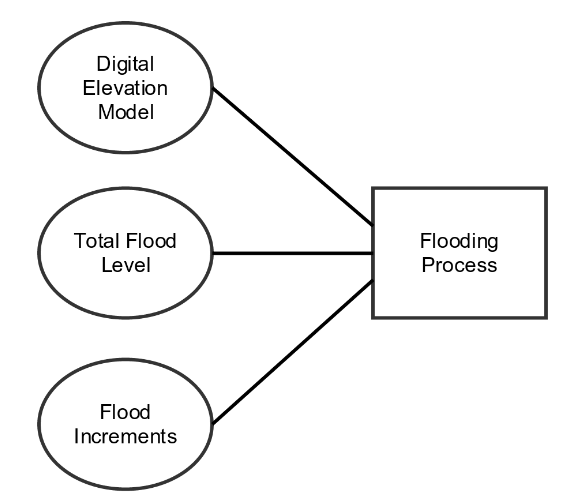
\includegraphics[width=.45\linewidth]{gfx/Phase_2/image.png}}
\caption{Inputs for the flooding model.}
\label{fig:inputs}
\end{figure}\\

\autoref{fig:inputs} is an attempt at showing the inputs used for the previous project. As can be seen only one external data source is required - a DEM. According to the LOCATION used within GRASS, every imported DEM has to have a WGS 84 geographical projection. An important factor of the model, is that all web-mapping operations are done on Open Street Map, which uses a slight variant of WGS 84 as well. As is mentioned in theory, GRASS uses GDAL for importing several type of raster maps and OGR for importing vector datasets. Taking the advantage of these modules it is possible for the to use any raster, as long as it is project into WGS 84. Another input of the model is the maximum flood level and the water rise increments of flood. These numbers define the amount of loops necessary before the flooding is complete.\\
To flood the DEM, the model extracts those areas that are below current level of the iterator (and therefore flood). The first iteration will always be the sea level, where the actual flood level is 0. This extracts every cell with a value of zero.  \\
This method will extract \emph{ALL} areas that have a value of 0, which usually will generate several disconnected clumps of cells, located in different areas of the DEM. As our model has to generate a flood from one specific area (so as not to simulate that all streams and lakes in an area are filling with water) the model will require that the user interacts further. The user needs to choose from which source he/she would like flood the DEM from. The pre-selected point has a major role in this part of the model, as the flooding will be based on it. \\

After extracting every cell that is below the actual flood level, the process runs a cost distance analysis using the point as a source. The returned raster shows only one continuous area, for that level of the flood. The output cost raster is then converted to a vector with the value of the flood level. Each iteration extracts the land from the raster which is below the current flood level and select the continuous area depicting the actual flood on the land from the preselected source. 

The process is illustrated on \autoref{fig:continuous}. On \autoref{fig:allflood}, the algorithm identifies every possible cell that is under the current water level, indicated by the pink color. After the r.cost module has finished, the process returns a layer indicating which cells are reachable, as seen on \autoref{fig:actualflood}.\\

\begin{figure}[h!]
  \myfloatalign
  \subfloat[Every cell with a value less than the current flood level.]
  {\label{fig:allflood}  
  {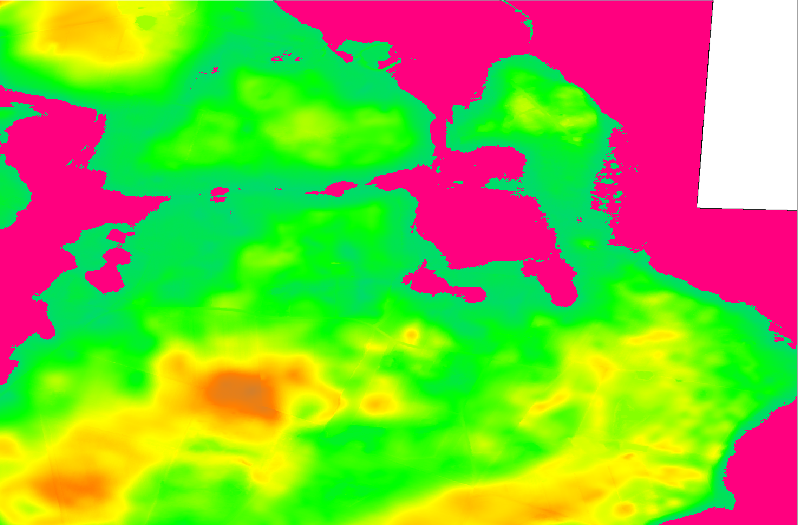
\includegraphics[width=.45\linewidth]{gfx/Phase_2/image2.png}}} \quad
  \subfloat[Cells reachable from the source point.]
  {\label{fig:actualflood}%
   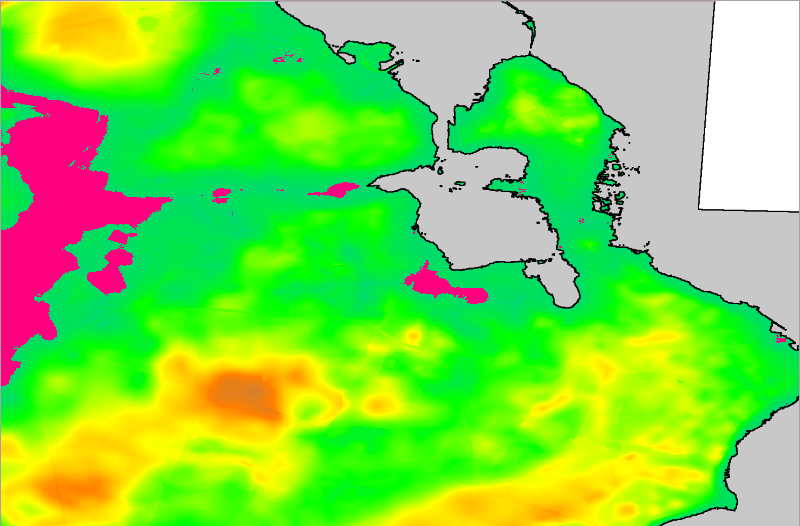
\includegraphics[width=.45\linewidth]{gfx/Phase_2/image3.png}} \\
 \caption{Figures indicating how r.cost is used to identify continuous areas}
 \label{fig:continuous}
\end{figure}

Every complex module from the earlier project has been taken out, and it has been simplified by using basic geoprocessing tools such as rasterizing, vectorizing, raster calculator and cost analysis. After the python - GRASS conversion was done, additional functionality was created, which will be discussed in \autoref{ch:phase4}.

\subsection{Problems encountered}

From the very beginning we were planning on using cost distance as the basis of our flood model, but we developed a different solution for the flooding algorithm, which turned out to be problematic – a problem we will address later in this section. The intent was to substitute the cost distance function with a more simple, and significantly faster, method. The procedure entailed spatially selecting only the extent which is connected to the source vector feature. The process is mostly the same, however instead of running the cost distance function, the extracted areas are converted to vector polygons and by using an intersect tool (v.select), only the polygon which is intersected with the pre-selected vector point is selected, this can be seen from \autoref{fig:phase2_prob1}\\
It can be seen, the red polygons represented all areas, which can be a possibly flooded with a 1.2 meter water level, however these areas are widely spread along the investigated area. The selection is  based on the user's pre-selected the flood source, which is the yellow cross in the figure. The GRASS module select the intersecting flood polygon, which represents only that stage of flood, which have the connection to the source, illustrated by the blue polygon on \autoref{phase2_prob2}. 

\begin{figure}[h!]
  \myfloatalign
  \subfloat[Every cell with a value less than the current flood level.]
  {\label{fig:phase2_prob1}  
  {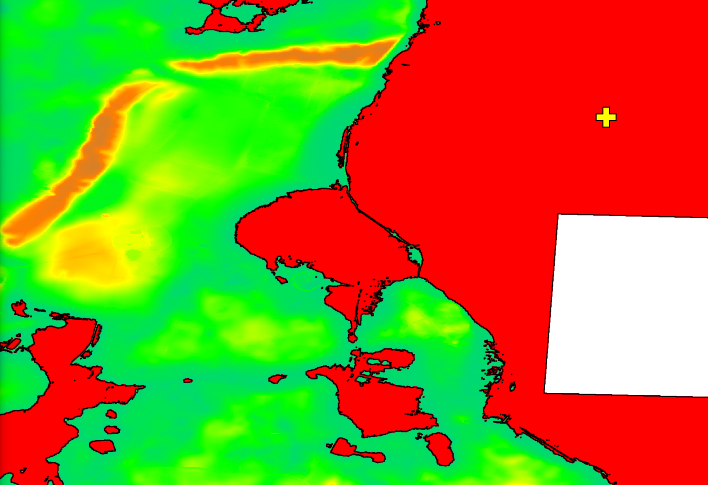
\includegraphics[width=.45\linewidth]{gfx/Phase_2/problem1.png}}} \quad
  \subfloat[Cells reachable from the source point.]
  {\label{fig:phase2_prob2}%
   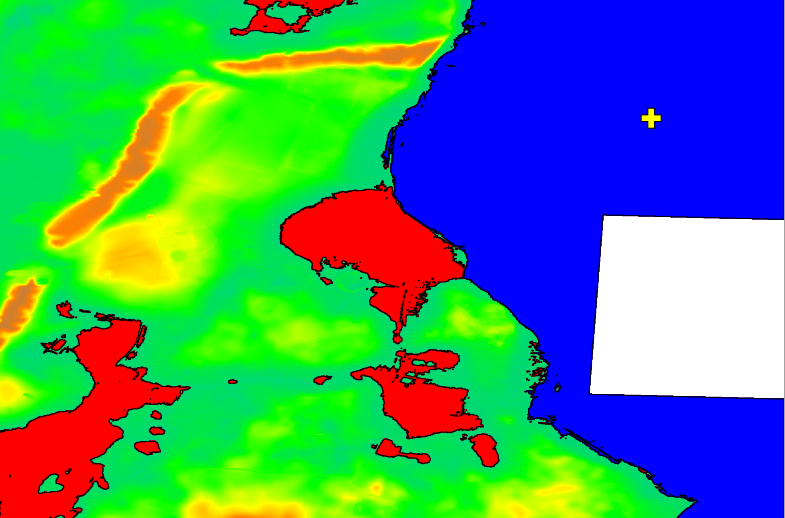
\includegraphics[width=.45\linewidth]{gfx/Phase_2/problem2.png}} \\
 \caption{Figures indicating how r.cost is used to identify continuous areas}
 \label{fig:phase2_prob12}
\end{figure}

\paragraph{Cost Distance vs Spatial Selection}

Comparing the cost distance and the spatial vector selection methods, the following problems and drawbacks appeared. According to our tests with the two process, we realized that the processing time was significantly greater with the cost distance function, because of it's cell by cell calculation. So larger grids imported to the process will increase the processing even more, due the increased amount of cells. At the end of the development stage we realized that the spatial selection did not behave in the same was as the r.cost functionality does. As it described earlier, the spatial selection selects only the polygon connected with the source. Since the vectorizing is done based on the cell resolution, if a cell is only diagonally connected to the “coherent” area, than it will be allocated as a different polygon, as presented on \autoref{fig:phase2_prob3}.

\begin{figure}[h!]
\centering
	{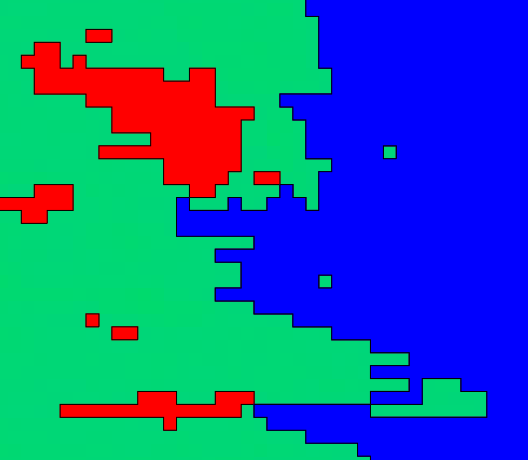
\includegraphics[width=0.8\linewidth]{gfx/Phase_2/problem3.png}}
\caption{Inputs for the flooding model.}
\label{fig:phase2_prob3}
\end{figure}\\

Therefore every cell, which is diagonally connected to a coherent flood surface will be disregarded, even though they, according to the flow direction and accumulation theory, would be the part of the flood extent. 
We tested both functions have confirmed a significant impact on the results of the process. For example, comparing a flood scenario of 3 meter flood rise with 10 cm increments, it can be seen that at stage 1,20m, the flood extent is significantly different, as seen on \autoref{fig:phase2_prob4}

\begin{figure}[h!]
\centering
	{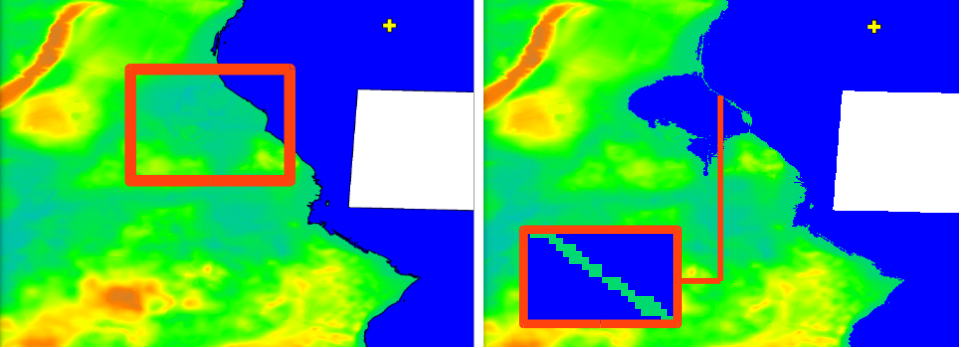
\includegraphics[width=\linewidth]{gfx/Phase_2/problem4.png}}
\caption{Inputs for the flooding model.}
\label{fig:phase2_prob4}
\end{figure}\\

\section{Phase 3}
This section will focus on the back-end of our web server. We begin by initializing Flask on our server. It is important to keep in mind that we earlier installed the Apache web server. After extensive research online, several different sources suggested a universal process on how to install Flask on an Apache 2 server. To go on, before actually installing Flask, we need to initialize mod\_wsgi. Mod\_wsgi is a tool that specializes in serving python applications from Apache servers. Installing mod\_wsgi is quite easy, and only takes a few lines of command line scripting (figure XXX).\\

\begin{lstlisting}
sudo apt-get install apache2 apache2-base apache2-mpm-prefork apache2-utils libexpat1 -ssl-cert
sudo apt-get install libapache2-mod-wsgi python-pip git
pip install flask
\end{lstlisting}\\

Following this installation we need to create an application.wsgi file. This is basically a file that contains code that initializes the application and comes with the .wsgi file extension. 
Now that Flask and prerequisites have been set up, it is time to look at what the backbone of the application looks like. At first, it is important to mention that the initial setup of the application will use Flask. To start with, and keeping in mind the way Flask actually works, we need a main Flask script that can initialize the application and connect various functions with its main core. In addition, that main script will also be connected to various html pages depending on where the user wants to navigate in our application.
The first action we took was to change the default path of our application in the server. Instead of using \textit{/var/www/html}, we started using \textit{/var/www/html/FlaskApp/FlaskApp}. This path will be referred to as the root url. After doing that, we create the script that will perform the functionalities of the application. That script is named \_\_init\_\_.py. Using Flask allows us to connect to various html scripts by using  only one main script. Depending on the URL of the page the user wants to get to, the corresponding HTML script is called and displayed on the user's screen. For example, as shown below (figure XXX), if the user visits our homepage, which is set by the \textit{\@app.route()}, then the \textit{'index.html'} will be initialized and displayed on his screen.\\

\begin{lstlisting}
@app.route('/')
def hello_world():
	return render_template('index.html')
\end{lstlisting}

The first action the user must perform in order to begin using the application is to upload a DEM. When the user clicks on the FLOOD button on our starting page, they get redirected to the root url/upload  section of the application. The way that section is working is that it expects a file to be posted. When that happens, it saves it to a pre-designated folder on the server. Right after that, we create a copy of the uploaded file and convert it from .tiff to .png. The reason behind that conversion is that we need to display the uploaded elevation model on a map for the user to see, which is vital to the next steps of the application. In order to be able to overlay an object on top of a map using leaflet, then that object has to be of .png or .jpeg format. All the aforementioned functions are included in the script below.\\

\begin{lstlisting}
def upload_file():

	if request.method == 'POST':
		file = request.files['datafile']
		if file:
			filename = secure_filename(file.filename)
			file.save(os.path.join(app.config['UPLOAD_FOLDER'], filename))
			src_ds = gdal.Open( os.path.join(app.config['UPLOAD_FOLDER'], filename) )
			formatimage = "PNG"
			driver = gdal.GetDriverByName( formatimage )
			fileName, fileExtension = os.path.splitext(filename)
			finalloca = '/var/www/html/FlaskApp/FlaskApp/static/images/' + str(fileName) + '.png'
			dst_ds = driver.CreateCopy( finalloca, src_ds, 0)
\end{lstlisting}

When the upload process is complete, a function is initialized allowing us to display that image on the map. Since we are using leaflet as a javascript library, in order to be able to display an image, we need to provide the function with the coordinates of the South-West and North-East corners of the image's display boundaries. To acquire this piece of information, we use gdal. The way we obtain the required coordinates are show below.\\

\begin{lstlisting}
			width = ds.RasterXSize
			height = ds.RasterYSize
			gt = ds.GetGeoTransform()
			minx = gt[0]
			miny = gt[3] + width*gt[4] +height*gt[5]
			maxx = gt[0] + width*gt[1] + height*gt[2]
			maxy = gt[3]

			return redirect(url_for('upload_file',filename=filename,minx=minx,miny=miny,maxx=maxx,maxy=maxy))
\end{lstlisting}\\

The final step we need to take before we are able to show the uploaded image, is to pass coordinates back to the html document that is responsible for showing that image so that a javascript function can get and display the image properly. That is achieved by the final line of the script on the image above.

\subsection{Problems encountered}
Having presented a viable option on how our web-service is structured and what tools we used to achieve successful functionalities, it is time to examine what other alternatives we have explored that did not result in acceptable results.\\
As presented above, we use Flask to create the back-end of our application. This decision was not our initial one, since none of the group members  had any particular experience using this framework. That being said, it normally would seem a rather unorthodox approach to start using a tool that no one is familiar with at the middle of our project development, since that is when we introduced Flask to the project. The truth is that our first option was to use an HTML and JavaScript core and PHP to upload the user provided input to the application. To be more specific, we would have an HTML document that allowed the user to upload a file and use PHP to convert that file from .tiff to .png. Then that PHP script would call a python script that calculated the bounding box coordinates of the image and then pass them on to a second HTML document, to be used by a JavaScript function that overlays the image on the map. The reason we considered using that approach is that we were more accustomed to using PHP to perform specific functions such as manipulating and uploading a file. On the other hand, this approach is clearly much more complicated than the one we finally used. Especially, if we keep in mind on how many different programming languages are included in that approach and how many different scripts we need to connect in order for it to work.  In addition, the transition from PHP to python was never achieved up to the point where we decided to change directions.\\

What we managed by using Flask instead, was to exclude the use of PHP and thus reduce the complexity of the script by a great deal. Firstly because we do not have to worry about creating extra connections with various other scripts. In fact Flask, and the way it is designed to operate, simplified our development considerably. It allowed to have a central script of python that inherently interconnected with all our HTML scripts and supported other python functions at the same time.

\section{Phase 4}
\label{ch:phase4}

To expand on the functionality of the application, we have additional functionalities and tools, which could be a tool used for flood or disaster management. 

\subsection{Identifying critical areas}
\subsubsection{Outlet analysis}
During the development of the pour-point analysis, we encountered sine problems. At the beginning, we tried to derive this problem from a watershed analysis, based on the identification of watershed's outlet. Our hypothesis was , that the flood  would flow backwards through the flow accumulation and flow stream model to the source cells and when the water enters through an outlet, to a new watershed, than that area would become flooded. Therefore we created a workflow which extracts only the outlet of the watershed. As it presented in the theory part, we used the watershed(r.watershed) and flow accumulation module (r.terraflow) in order to determine the inlet-outlet location of the watershed. We tried to establish an algorithm for relative watershed determination based on the investigated DEM. We set up, the minimum threshold size of a watershed, has to be at least the ten percent of the DEM. After the workflow run the previously used neighborhood analysis(r.neighbor) with diversity method with we could extract the watershed borders on a raster. Using the terraflow module with single flow direction setup, we created the a flow accumulation raster. This is important to determine the inlet/outlet location. Using the single flow direction method, every outlets will be located on the border of a watershed where the flow accumulation is the maximum. With this approach we though we got can a relatively good result to determine where the flood flow will enter to new area, however the testing of the algorithm showed its failure of our planned purpose.

\subsubsection{Pour point analysis}
Only providing the a extent is not enough when wanting to prepare against the impact a disaster. We wanted to provide more information about the flood regarding areas that might be particularly dangerous. After monitoring the  spread of the flood using our simple model, we realized there were areas where a relatively large area got flooded immediately. This can occur when the flood steps over a natural barrier, with a lower elevation than the surrounding area. This is what we call a “pour-point”. One of our major challenge was how to identify this behaviour and to locate the actual position of these critical points automatically.// 
Since these pour point phenomena are very dependent how the process is run; which increment the water is rising in; which output (raster or vector) are we working with. Firstly, we realized that to give an accurate flooding the increments would have to with 1 cm water increments. By using this increment, this flood can be accurate enough to identify major changes between consecutive flood levels.

\begin{figure}[h!]
\centering
	{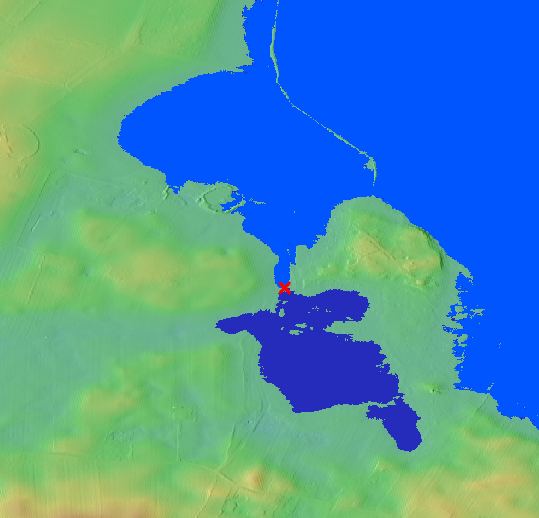
\includegraphics[width=0.80\linewidth]{gfx/Pourpoint.png}}
\caption{Figure showing the pourpoint we are trying to identify.}
\label{fig:pourpoint}
\end{figure}

\autoref{fig:pourpoint} shows two consecutive flood extents with 140cm(light blue) and 141 cm (dark blue) water rise. The red area indicated on the figure is what we needed to locate. Although it might seem to be a fairly easy procedure, we have to add that the large blue area on the image is not the only area that has increased in size between the two stage of flooding. Along the border of 140 cm (light blue) flood level, there are a relatively small areas or cells  which are flooded at the 141 cm. In order to avoid small or irrelevant pour point identification the following workflow was created. 
As described in phase 2, after each flood extent the output is stored in both raster and vector format. In order to overcome the situation to identify pour points at each level, we implemented a condition which checks the size difference between each consecutive stage. We added an area field for each flood extent polygon, thereby we can built a decision analysis based on the flooded area. If the difference between two consecutive flood stages is larger than one percent of the investigated DEM, then the pour-point analysis workflow is triggered. The two investigated flood extents are subracted from each other, a selection based on its area field is conducted. By performing this subtraction, a lot of polygons are created. For each polygon the process calculates an area field and selects only those that are larger than 1000 square meters. This criteria is to avoid relatively small areas (indicated in grey on \autoref{fig:twofloods}, which the pour point analysis would not make a reasonable investigation since their size is negligible compared to those area which have a larger impact on the advancing of the flood (indicated by the red color) . After the exclusion, only those areas which have a larger extent than the previously mentioned criteria are left.\\

\begin{figure}[h!]
  \myfloatalign
  \subfloat[Showing two flood extents.]
  {\label{fig:twofloods}
  {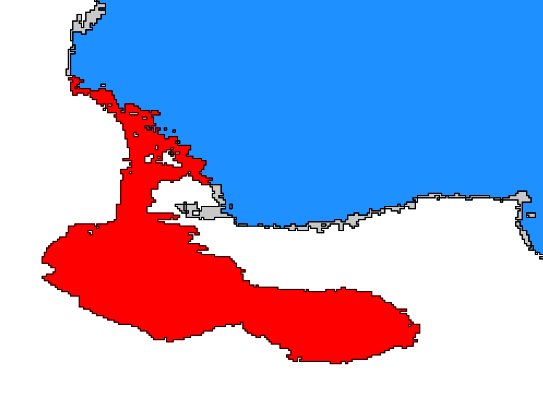
\includegraphics[width=.45\linewidth]{gfx/Phase_4/Pourpoint2.png}}} \quad
  \subfloat[Showing line of pour points.]
  {\label{fig:allthepoints}
   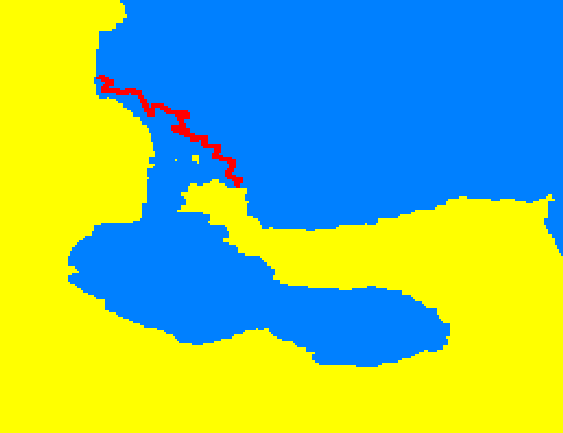
\includegraphics[width=.45\linewidth]{gfx/Phase_4/Pourpoint3.png}} \\
  \caption{Showing the concepts of finding the pourpoints.}
  \label{fig:pourpoints}
\end{figure}

The remaining polygon(s) are converted back to raster and merged with the previous raster extent of the flood, thereby a new raster map represents, the previous flood (blue) and the actual flood (red) with increments which are over the criteria. This raster has raster values where the flood extent exists and NULL values everywhere else.
Afterwards a neighborhood analysis (r.neighbors) is conducted, based on the diversity method – which is based on the Moore-Neighborhood. This method is applied in order to find the location, where the raster changes values, since that place is where the flood enters into the new area. In \autoref{fig:twofloods} a black border can be seen, where the red and blue area touch. The process need to identify automatically only that border which connects the two different flood stage in the critical location – I.e the pour points. The diversity method can be used to identify only the border cells as it seen in \autoref{fig:allthepoints}.
After the identifying the pour-point cells with the above-mentioned analysis, the algorithm then extracts those cells and converts them to vector points. \\

To have the pour-points as vector points is partly because we can then easily store information about the necessary height of a barrier at this place, and so that they easily can be displayed and manipulated on our web map following the analysis procedure. 
For the better understanding and providing essential information of the critical area, we decided to add th elevetion of the pour-point location and the maximum flood depth based on the actual scenario. This was done by point sampling method of GRASS. (r.what.rast). Sampling method extracts those cell attribute, where the vector points act as a centroid of the cell square. \\

\subsection{Barrier placement}
An integral part of the application is allowing the user to implement barriers that will mitigate the effects of the flood. The user will be able to determine whether an area can be secured by the implementation of obstacles in the landscape or how the flood can be affected by installing a barrier in a given position. \\
The general operation of having the barrier placement process available to the user starts after the flood simulation has been performed and completed. This is because the user has to have an overview of the overall situation of the flood and the location of the critical areas in the landscape, before starting placing barriers in random areas and in an arbitrary fashion. We believe that this would ensure that the entire process of finding a suitable solution to a flood situation is fast since performing the advanced simulation can take a lot of time.\\

The process begins by getting the input from the webpage where the user draws a barrier on a web map. This results into the creation of a GeoJSON file that is then transferred to the python function that creates the does the modelling. Since the barrier is in GeoJSON format, we need to convert it to raster in order to hardcode it into the elevation model. Normally, converting the barrier to raster and then adding it to the elevation model would be enough. Unfortunately, we stumbled upon a quite unexpected problem. The sections of the barrier that are not completely vertical or horizontal are rasterized in an erroneous fashion. To be more specific, in these sections the cells are not connected with a shared side of cell. Instead, they are connected by sharing an edge. The figure below demonstrates the problem when the barrier is converted to raster, as can be seen in \autoref{fig:rasterize}.\\

\begin{figure}[h!]
  \myfloatalign
  \subfloat[Rasterized barrier.]
  {\label{fig:rasterize}
  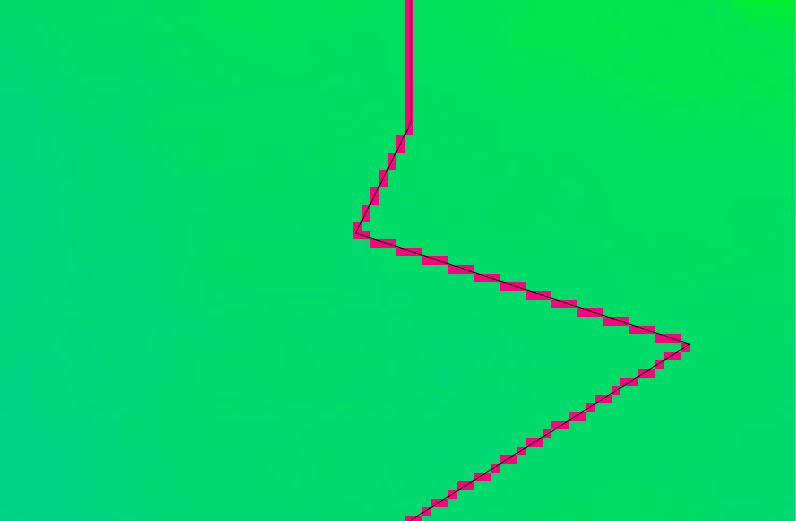
\includegraphics[width=.45\linewidth]{gfx/Phase_4/Barrier1.png}} \quad
  \subfloat[Problem areas.]
  {\label{fig:problemareas}%
   
\includegraphics[width=.45\linewidth]{gfx/Phase_4/Barrier2.png}} \\
  \subfloat[Generating pixels in the designated areas.]
  {\label{fig:barrier3}
  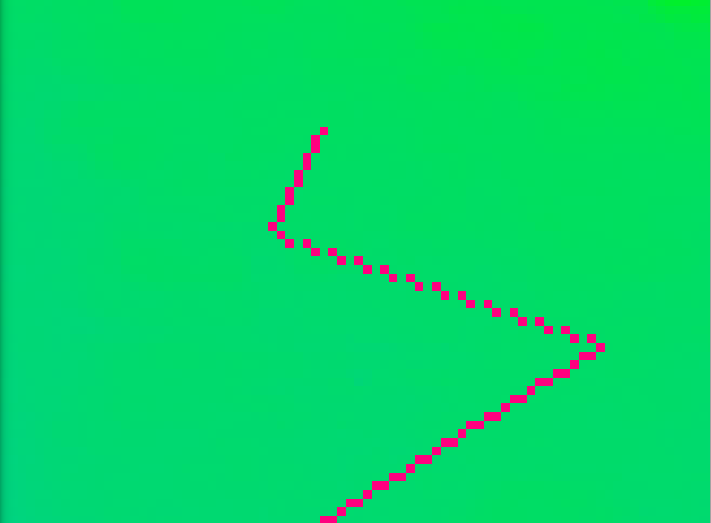
\includegraphics[width=.45\linewidth]{gfx/Phase_4/Barrier3.png}} \quad
  \subfloat[Fixed barrier.]
  {\label{fig:barrier4}
  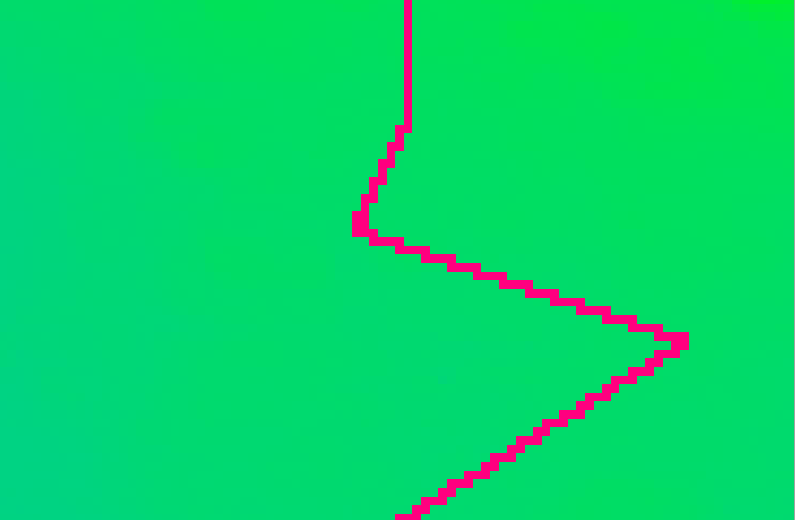
\includegraphics[width=.45\linewidth]{gfx/Phase_4/Barrier4.png}}
  \caption[Generated extra pixels]{The process of fixing the rasterized barrier.}\label{fig:barriers}
\end{figure}

The problem depicted above is quite unexpected especially if we take note of that fact that the conversion ignores several cells that intersect with the barrier line and instead keeps only cells that are connected diagonally with each other. That leads to gaps on the barriers that would allow water to flow through them. In order to deal with that problem we have developed the following solution. \\
Practically, we need to assign the pre-designated value of the barrier height to one of the cells per diagonal intersection to create a continuous raster of the barrier, as indicated on \autoref{fig:problemareas}. 

In order to do that, first we extract the edges of the non-vertical, non-horizontal sections of the barrier. In addition, we extend those cells by one cell in the northerly direction. That action is performed by the following part of the script, as seen on \autoref{fig:barrier3}.

\begin{lstlisting}

\end{lstlisting}

As can be noted in the script above, we are using neighborhoods in order to extract the necessary cells. In fact, we are not using full neighborhoods (e.g. Moore Neighborhood) but specific cells that exist in the neighborhood of the cell mapcalc is actually querying. In order to query the correct cells, we are required to know their relative coordinates to the center cell that is queried. These relatives coordinates are displayed on \autoref{tab:relcoord}.\\

\begin{table}
\centering
\begin{tabular}{l | c | r}
-1,-1 & -1,0 & -1,1 \\
\hline \\
0,-1 & 0,0 & 0,1 \\
\hline \\
1,-1 & 1,0 & 1,1 \\
\end{tabular}
\caption{Relative cell coordinates to the center cell (0,0)}
\label{tab:relcoord}
\end{table}\\

The result of this edge selection is shown on the figure below (figure XXX).\\
\\


Since we have the edges of the barrier, we go on by expanding each one by one cell, as mentioned above, and merge the resulting raster with the initial barrier raster. That is done with the following script:\\

\begin{lstlisting}
gscript.run_command('r.patch', inputs=['edges_1_1_ext','edges_11_ext','barr_raster'],output='merged)
\end{lstlisting}\\

The final step in order to complete the barrier correction and deployment to the landscape is to hardcode it to the elevation model. Which is done with the following script: \\

\begin{lstlisting}
gscript.run_command('r.mapcalc', expression='original_b = if(isnull(merged),original,original+merged)')
\end{lstlisting}

This process results in the elevation model shown on \autoref{fig:fixedbarrier}.

\begin{figure}[h!]
\centering
	{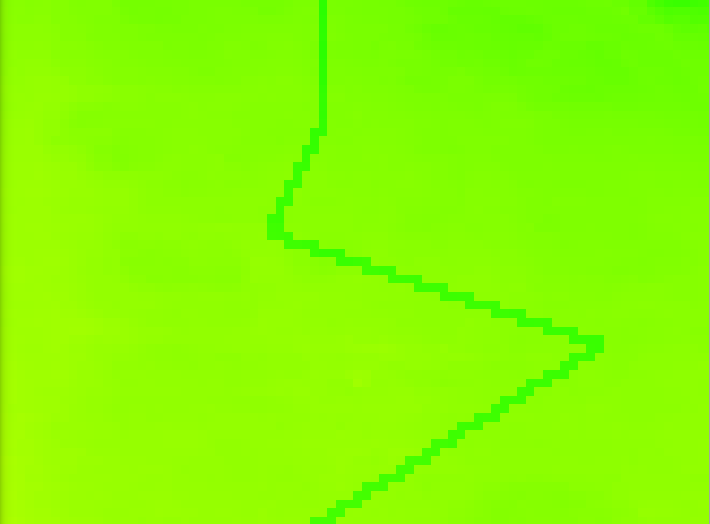
\includegraphics[width=0.75\linewidth]{gfx/Phase_4/Barrier5.png}}
\caption{Figure showing important concepts when working with watersheds}
\label{fig:fixedbarrier}
\end{figure}

By observing the result above, someone might think that it is difficult to observe the actual barrier and distinguish it from the elevation model. Unfortunately, this is the result of merging the two rasters together. It is logical that the results are not visually distinctive since they are in fact one raster represented by a sliding color scale.

\subsection{Problems encountered}
The main issue with the process of creating the barrier and performing the necessary correction was the necessity of actually performing the correction of it. That means that normally, the conversion of a linear vector file to raster should not behave the way we described above. we assumed that GIS software suits, such as QGIS and GRASS as well as ArcGIS, address issues as connectivity of cells in identical fashion. But unfortunately that was not the case. In fact, ArcGIS considers cells that share an edge (diagonal connection) as connecting cells and will include them in a raster to vector conversion. On the other hand, QGIS and GRASS does not. This lead us to dedicate a considerable amount of time in creating a solution.\\

Another issue that we faced was the lack of documentation on the mapcalc function that we used in this process. Despite following the existing documentation closely, we ran into problems that should not have existed. Initially, the proposed solution to the barrier problem consisted of a much more compact script that performed a universal query on all the cells of the barrier raster in order to cover its gaps. Unfortunately, for reasons yet undiscovered, that solution did not produce any results. The script we used can be seen below at its final state before we decided to develop the solution that performed as expected.

\begin{lstlisting}
corr_barrier = if(isnull(barr_raster), if(barr_raster[0,-1] == 3 && (barr_raster[-1,0] == 3 || barr_raster[1,0] == 3) , barr_raster, null()) || if(barr_raster[0,1] == 3 &&  (barr_raster[-1,0] == 3 || barr_raster[1,0] == 3), barr_raster, null()), barr_raster)
\end{lstlisting}

\section{Phase 5}
This phase involves setting up the necessary website relevant elements. This means both HTML, Javascript, web mapping and the understanding of PyWPS.\\

\paragraph{PyWPS:} As the the main functionality of our script was developed, we began porting the script to PyWPS syntax. 

The output cannot be defined dynamically. 

As mentioned in the theory part, every PyWPS must include 
\begin{itemize}
\item \_\_init\_\_ 
\end{itemize}
and 
\begin{itemize}
\item execute.
\end{itemize}
  
The various settings we set up to be:

\begin{itemize}
\item identifier = "flooding",
\item title = "Flooding",
\item abstract = "This process is used to flood a DEM with water",
\item version = "1.0",
\item grassLocation = "/home/ubuntu/grassdata/WGS\_1984",
\item statusSupported = True,
\item storeSupported = True
\end{itemize}

The most un-intuitive of these settings are the \textit{grassLocation}, \textit{statusSupported} and \textit{storeSupported}. 
We set \textit{grassLocation} to our predefined database folder. This is done in order to make sure that the uploaded data will work within a coordinate system, and that we can do the proper calculations on it.
When setting \textit{statusSupported} to True, means that the process can run asynchronously. 
And finally, using \textit{storeSupported} means that it is possible to deploy the results to the server, for later usage. 
After this has been set, we define the needed inputs. As mentioned previously, we want the user to provide a DEM and a point indicating where the flooding should occur from. Therefore we must inform the program that we will be expecting an image and a GeoJSON file. 

\begin{lstlisting}
self.rasterin=self.addComplexInput(identifier='rasterin',
		   title="input image",
	   	   formats = [{'mimeType': 'image/tiff'}, {'mimeType': 			             	'image/geotiff'}, 	   {'mimeType': 'application/geotiff'}, 		            {'mimeType': 'application/x-	   geotiff'}])
	   	   
self.vectorin = self.addComplexInput(identifier="vectorin",
		     title="Input point",
		     formats = [{"mimeType":"text/json","encoding":"utf-			              8","schema":None}])

\end{lstlisting}

After having defined the inputs. It's is also necessary to define the outputs. We want to provide the user with a raster of the flooding and the extent of the flooding as a vector file. Furthermore, after the process has completed, we want to provide an in-browser image of how the actual flooding looks. Because very few browsers natively support the display of TIFF images, we will output a JPEG as well:\\


\begin{lstlisting}
self.outputImage0=self.addComplexOutput(identifier="output0",title="output image", asReference=True)

self.outputImage1=self.addComplexOutput(identifier="output1",title="output image", asReference=True)

self.outputVector=self.addComplexOutput(identifier="output2",title="output vector", asReference=True)

\end{lstlisting}

By setting the setting \textit{asReference} to True, the output will not be delivered straight back to the user, but will be provided as a link to the location in which it is stored on the server. When returning images with PyWPS they get delivered as Base64 images, which means that they are returned as a long string of text. This can reduce the loading times significantly, and can for very large images also freeze the computer handling them. Furthermore it has the advantage, that if a user should lose connection, the images can still be recovered. 

Now that the initialization settings have been defined, the execute method can be set up. In general the code looks very similar to the functions created earlier, so they will not be explained here further (and they can be found on the previously mentioned GitHub page). 
After creating the service, they are placed in the processes folder on the server. Furthermore the \_\_init\_\_.py file is updated to now include the uploaded file. 
After having set up the script in PyWPS, and transferring them to the server, they are reday to be called. This can be done through the web browser.
In general it is possible to call either a GetCapabilities, Execute or DescribeProcess. For this project it will only be necessary to Execute a process, as this project is not meant to be accessed outside of our webapplication interface. 
They way the WPS service is requested from the server, I.e a flooding service with the identifier “flooding”, is called like follows:

\begin{itemize}
\item http://52.17.144.192/cgi-bin/pywps.cgi?request=execute&service=WPS&version=1.0.0&identifier=flooding&datainputs=[rasterin=<LINK TO DEM>;vectorin=<GEOJSON AS STRING>]
\end{itemize}

The server will process the request, and return a XML document with links to where the outputs of the process are stored. 

\paragraph{Setting up the design:} Using the power of Flask as much as possible, we wanted to make the website have as small of a footprint as possible. 
The application would consist of a welcome page with a brief introduction which would link the user to the “actual” application, which would be followed by a multi-layered page, that would guide the user through the process of flooding. 
IMAGE OF FRONTPAGE → IMAGE OF UPLOAD
Using the free Twitter Bootstrap CSS theme, it is possible to quickly create some working HTML pages. 

As the front page mostly contains information about the projects capabilities, this part will mostly focus on the second page. 

To guide the user through the process of flooding, it was decided to split the entire process into three steps:
\begin{itemize}
\item Step 1: Upload DEM
\item Step 2: Select Ocean
\item Step 3: Get Results
\end{itemize}
The three steps consist of various HTML parts that are hidden from the start, and as the user clicks through the steps, the next one is shown and the previous one is hidden. This is done using the following jQuery commands:

\begin{lstlisting}
$.(#step1).hide();

$.(#step2).show();
\end{lstlisting}

At most of the stages, asynchronous requests or operations will be performed. As they can take some time, we want to give the user some feedback that the page is loading. This is done by creating an overlay that takes up the entire screen, and includes a loading icon. The icon is hidden, but gets shown when a request is performed, in the same manner as above.
To describe how the outlined stages work we will go through them below. 

\textsc{Step 1 – Upload DEM:}
In this step the user uploads a DEM. Most of the functionality here is dependant on the functionality of Flask. So the only thing necessary to add here, is a HTML form with the capability of letting the user browse his computer for a DEM, and then clicking a button to upload it. 

\textsc{Step 2 – Select Ocean:}
In this step we want the user to select from where the flooding will occur. 

This entails showing the uploaded image on a webmap, making the user able to place a marker on the map, and then sending this information to the server.

When the upload has completed, the page refreshes. This means that the page clears all set variables. This is an issue when wanting to stay on the same page, but to load a different step. As Flask adds a variety of variables to the URL of the page, a workaround for this problem is to check to see if the URL contains  one  of the variables assigned by the Flask upload script:

\begin{lstlisting}
url = window.location.href;

if (url.indexOf("filename") > -1); {
	STEP 2

\end{lstlisting}

As mentioned, we want the DEM to be uploaded to a webmap. To do this a copy of the uploaded is created as a JPEG, which then can be used to overlay on the map. The JPEG cannot contain embedded coordinates. Using Flask, the corners of the uploaded TIF are extracted, and get returned to the URL of the webpage.
The format of this is something like:

\begin{itemize}
\item http://52.17.144.192/upload?minx=COORD&miny=COORD&maxx=COORD&maxy=COORD&filename=FILENAME
\end{itemize}

To extract the relevant data the following JavaScript code is executed:

\begin{lstlisting}
var findcorners = url.replace("http://52.17.144.192/upload?");
var findcorners2 = findcorners.split("&")
var filename = findcorners2[4].split("=")
var coordinatesforuse = [];
var expendable;
for (var i = 0; i < findcorners2.length; i++) {
    expendable = findcorners2[i].split("=")
    coordinatesforuse[i] = expendable[1];}
These are then stored into variables with a readable format:
var south = coordinatesforuse[0];
var west = coordinatesforuse[1];
var north = coordinatesforuse[2];
var east = coordinatesforuse[3];

\end{lstlisting}

Lastly they are prepared for insertion as the bounding box for the uploaded image, into the leaflet map:


\begin{lstlisting}
imageBounds = L.latLngBounds([
      [west, south], // Southwest
      [east, north] // Northeast
]);
\end{lstlisting}

As the uploaded TIF is converted into a PNG, but not returned to the URL, we are manually going to setup the URL where the PNG version of the uploaded image can be found:

\begin{lstlisting}
var imageuse = filename[1];
var imageaspng = imageuse.replace(/\.[^/.]+$/, ".png")
var variable = 'static/images/' + imageaspng;
var imageUrl = variable;
\end{lstlisting}

Now that all of this is done, we can initiate our map. Add the uploaded PNG as an overlay to our MapBox image, and define the marker that will be used.   

\begin{lstlisting}
// Initiate map "around" the uploaded DEM
var map = L.mapbox.map('map', 'piratosthegreat.i7aeacaf').fitBounds(
imageBounds);
// Add the DEM to the map
var overlay = L.imageOverlay(variable, imageBounds).addTo(map);
// Define marker
var marker = L.marker([16.436673, 38.322712], {
		icon: L.mapbox.marker.icon({
		'marker-color': '#f86767'
    })
});
\end{lstlisting}

To make it easier to find the ocean underneath the overlaid image, a transparency slider is added. This slider is provided by MapBox and can be freely found in their documentation.

The final thing is to add the onClick functionality of adding a point when clicking on the map, and to be able to send it to the server as a GeoJSON. This was done as follows:


\begin{lstlisting}
   map.on('click', function(e) {
               marker.setLatLng(e.latlng).addTo(map);

               markercoords = marker.getLatLng()

               geoj = [{
                   "type": "FeatureCollection",
                   "features": [{
                       "type": "Feature",
                       "properties": {},
                       "geometry": {
                           "type": "Point",
                           "coordinates": [markercoords.lng,
                             markercoords.lat
                           ]
                       }
                   }]
               }];
           });
\end{lstlisting}

We decided to add the possiblity for the user to choose between two different types of flooding at this stage. Either to do a quick flooding simulation, or a more advanced flood.
As soon as the relevant button is clicked, an asynchronous request is sent to the relevant PyWPS service.

\textsc{Step 3 – Get Results:}
Because of the response document from the PyWPS service being the same for either call, the structure and functionality of the asynchronous request performed will be (mostly) the same for both requests. So therefore only one request will be described here. 
The buttons used to send the request have been marked with either a advancedflood or simpleflood ID. In this instance we wil look at the advanced flood async request.
We have stored the relevant PyWPS URL in a variable in our script, and we have replaced relevant input with the data uploaded by the user 

\begin{lstlisting}
var preconpath = 'http://52.17.144.192/cgi-bin/pywps.cgi?request=execute&service=WPS&version=1.0.0&identifier=flooding&datainputs=[rasterin=http://52.17.144.192/static/images/' + imageuse + ';vectorin=' + JSON.stringify(geoj[0]) + ']';
\end{lstlisting}

The request we will perform is a standard jQuery async request to the PyWPS by using \textit{\$.get()}. This is encased in a when and a done function as follows: \textit{\$.when(\$.get()).done();}

This sets the script up in such a way that, when the asynch request is done, it launches some other code. 
The when and async request code looks like the following:

\begin{lstlisting}
$.when(
$.get(xmlPath, function(xml) {
        $("#overlay").hide();
        $(".step2").hide();
        $(".step3").show();
// Find the elements in the response XMl that contain our data
        $("wps\\:ProcessOutputs", xml).find("wps\\:Reference")
         .each(function(i, value) {
                  var imagepath = value.getAttribute("href");
                   var imagepathbroken = imagepath.split("/");
                  outputimagearray.push(imagepathbroken[5])
});
}, 'xml')
)
\end{lstlisting}

What this does is to get the XML document returned from PyWPS, traverse it and for each result, store it in a variable called outputimagearray.
When this is done it takes the outputs stored in the above mentioned array, and adds them to the website as an overlay to a map, and with possibility of downloading them.

\begin{lstlisting}
.done( function() {
               $(".loading").append('<div class="map" id="map1" style="height: 		500px; width: 100%;">')
               var map = L.mapbox.map('map1', 'piratosthegreat.i7aeacaf')
               .fitBounds(imageBounds);

               var outputimagesimple = 'static/outputs/' + outputimagearray[1];

               var overlay = L.imageOverlay(outputimagesimple, 				imageBounds).addTo(map);

               overlay.setOpacity(1.0);

              var featureLayer = L.mapbox.featureLayer()
              .loadURL('/static/outputs/' + outputimagearray[0])
              .addTo(map);

               $(".loading").append('<form method="get" action="http://52.17.144.192/static/outputs/' + outputimagearray[2] + '"><button class="btn btn-success btn-lg btn-block" type="submit">Download data !</button></form>')
             });
});
\end{lstlisting}

\subsection{Problems encountered}
\paragraph{Currently does not work on Chrome:} The way the URL's are formed, with variables added to them, do not work well with Chrome- This is an issue that can probably easily be fixed, but during this process there was not time to discover how to solve this issue. 

\paragraph{It is not possible to overlay a TIF:}
It is not possible to overlay a TIF onto the Webmap, and as such we had to also create a copy of the uploaded file, as a PNG. This does not take a long time, but makes it more tricky to make the entire process work the way we intend it to.  

\paragraph{At the moment flooding can only occur from one place:}
The way the GeoJSON creation is set up, and the way that the marker gets added to the map, the flooding can only occur from one spot. This should be relatively easily remedied, but at the time of creation, it was deemed satisfactory that the flood could only occur from one location.
